\chapter[Projeto Estrutural]{Projeto Estrutural}

\section{Subsistemas Conectados ao Motor}

\subsection{Sistema de Arrefecimento}

	Quando se trabalha com um motor de combustão interna de um veículo, é importante saber que várias explosões são geradas dentro das câmaras de combustão. Levando isso em consideração, fica fácil assumir que essas explosões acabam elevando de maneira acentuada a temperatura de todo o sistema do motor. Por esse motivo, todos os veículos que possuem motores de combustão interna são equipados com algum tipo de sistema de arrefecimento. A função desse tipo de sistema é garantir que a temperatura do motor seja controlada em quaisquer condições operacionais utilizando conceitos de transferência de calor e garantindo que o calor gerado pelo motor seja dissipado no ar \cite{bosch2004}. Esse resfriamento do motor pode ser feito tanto com ar como com líquidos, embora na maioria das vezes os dois jeitos sejam utilizados juntos. 
	
	O sistema de arrefecimento é composto por um radiador, um ventilador, um conjunto de mangueiras de circulação, bomba d’água, termostato entre outros componentes que auxiliam no resfriamento do motor. 
	As funções de cada subsistema citado são:
	
\begin{itemize}
	\item \textbf{Radiador}: Manter a temperatura do líquido de arrefecimento que sai do motor em uma faixa aceitável de operação. O tamanho de projeto do radiador varia com a taxa de fluxo de ar- massa que entra no veículo e com a potência do ventilador.
	\item \textbf{Ventilador}: Os ventiladores, têm a função de apoiar o radiador realizando uma ventilação forçada de ar. É ativado muitas vezes por um sistema de correias ou eletricamente.
	\item \textbf{Mangueiras}: Transporte do líquido de arrefecimento até os dutos do motor e em seguida, da saída do motor até o radiador.
	\item \textbf{Bomba d’água}: Bombear o líquido por todo o seu ciclo de arrefecimento, garantindo um fluxo constante de água por todo o sistema.
	\item \textbf{Termostato}: Realizar medições de temperatura da água que passa por ele e verificar se o motor está operando na faixa desejada.
\end{itemize}

	O funcionamento do sistema de arrefecimento (Figura \ref{fig:sistemaarrefecimento}) consiste basicamente em um circuito fechado no qual a água circula em volta do motor realizando assim uma troca de calor com ele. Todo o sistema funciona com ajuda de uma bomba d’água que é conectada ao eixo do motor por uma correia. Enquanto o motor do carro ainda está frio, a água é circulada apenas em volta do motor. Uma vez que o termostato constata que a temperatura da água passou do valor considerado aceitável, uma válvula termostática se abre possibilitando assim que a água que estava circulando apenas em volta do motor se dirija para o radiador por meio das mangueiras. O radiador, feito de um material com boa condutibilidade térmica e posicionado na parte da frente do veículo, circula a água por um sistema de serpentina realizando assim uma troca mais eficiente de calor com o ambiente. Quando a água circula todo o radiador, ela retorna ao reservatório já com uma aceitável para ser recirculada no motor.
	
\begin{figure}[h!]
	\centering
	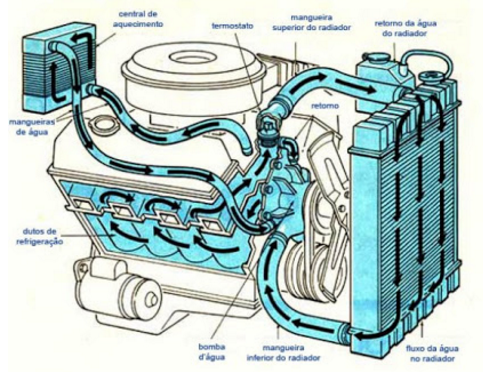
\includegraphics[keepaspectratio=true,scale= 0.7]{figuras/sistemaarrefecimento.png}
	\caption{Sistema de arrefecimento do Motor.}
	\label{fig:sistemaarrefecimento}
\end{figure}

\subsection{Sistema de Exaustão}

	Como o próprio nome já diz, o sistema de exaustão tem a função de retirar os gases resultantes das explosões de dentro da câmara de combustão \cite{heyood1988}. Esses gases uma vez que são retirados da câmara de combustão não podem ser jogados diretamente ao ambiente pois apresentam altas concentrações de poluentes como CO2, CO, NOx entre outros. Também existe a poluição sonora que é gerada pela explosão dos motores. Levando isso em consideração, os sistemas de exaustão em veículos apresentam um coletor de escape, catalisador e abafador. As funções de cada componente segundo o manual da \citeauthor{bosch2004} (\citeyear{bosch2004}) são:
	
\begin{itemize}
	\item \textbf{Coletor}: Direcionar o gás resultante das explosões na câmara de combustão de cada cilindro por orifícios em direção ao sistema de gás de escapamento.
	\item \textbf{Conversor Catalítico}: O conversor catalítico consiste em um funil em cada extremidade de fluxo e um suporte monolítico que é composto por diversos canais paralelos compostos por um revestimento catalítico ativo. Também existem os filtros de particulados que são basicamente filtros metálicos ou cerâmicos que possuem um grande número de canais paralelos e porosos que forçam o ar a passar por esses poros, fazendo com que as partículas sólidas fiquem depositadas neles. A eficiência de filtragem desse sistema pode chegar a até 97\%.
	\item \textbf{Abafadores}: Os abafadores tem a função de uniformizar as pulsações geradas pelos gases de escape de modo a silencia-las e torna-las as mais inaudíveis possível. Alguns abafadores já vem com o conversor catalítico integrado neles.
\end{itemize}

	O processo de exaustão é simples e rápido. Quando a válvula de escape é aberta, o coletor de escape transfere tudo que restou da combustão pelos tubos de escape até o catalisador. No catalisador, os gases nocivos a saúde são tratados de modo a diminuir ao máximo o efeito poluente deles. Em seguida os gases são transmitidos por toda a tubulação passando por um abafador de ruídos e um silenciador, ambos com a função de minimizar ao máximo a emissão de ruídos para o ambiente. Após passar pelo silenciador, os gases tratados são jogados ao meio ambiente. Esse processo é realizado toda vez que uma válvula de escape é abre. A Figura \ref{fig:sistemaexaustao} representa esquematicamente o sistema de exaustão de um veículo de passeio.
	
\begin{figure}[h!]
	\centering
	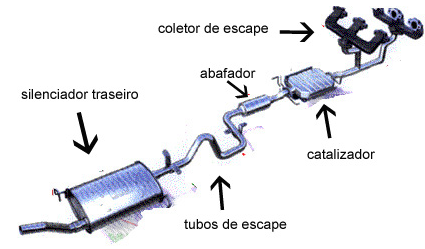
\includegraphics[keepaspectratio=true,scale= 0.7]{figuras/sistemaexaustao.png}
	\caption{Sistema de Exaustão.}
	\label{fig:sistemaexaustao}
\end{figure}

	Com os gases de escape é possível realizar uma medição precisa da mistura e concluir se ela está pobre, rica ou ideal. Em uma combustão ideal, ou combustão completa, todo o oxigênio e todo o combustível são queimados de modo que nenhuma reação secundária é gerada. Os subprodutos dessa reação de combustão ideal são água (H2O) e dióxido de carbono (CO2) \cite{bosch2004}. Por outro lado, a obtenção de uma combustão ideal é praticamente impossível visto que que existem diversas variáveis envolvidas neste processo. Quando uma combustão não é ideal, pode-se dizer que a mistura está ou rica ou pobre. Uma mistura rica significa que foi injetado mais combustível do que ar na câmara de combustão e portanto nem todas as partículas de combustível foram ligadas com as de oxigênio. A mistura é considerada pobre quando é injetado mais ar do que combustível na combustão e portanto nem todas as partículas de oxigênio foram ligadas com as de combustível. O efeito desses tipos de mistura é um número maior de subprodutos da reação que são gerados e por sua vez um número maior de poluentes dispensados no meio ambiente (Figura \ref{fig:efeitocatalisadores}). Os subprodutos de combustões incompletas podem ser monóxidos de carbono (CO), hidrocarbonetos (HC), óxidos de nitrogênio (NOx), oxidantes e particulados \cite{brunetti2012}.
	
\begin{figure}[h!]
	\centering
	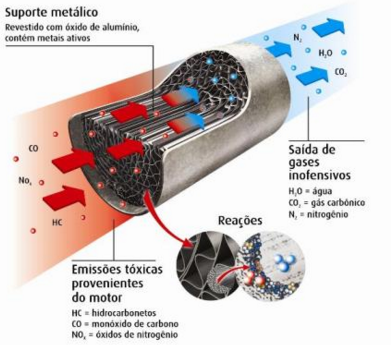
\includegraphics[keepaspectratio=true,scale= 0.7]{figuras/efeitocatalisadores.png}
	\caption{Efeito dos Catalisadores.}
	\label{fig:efeitocatalisadores}
\end{figure}

\subsection{Sistema de Lubrificação}	

	Em um motor de combustão interna, quanto menor o atrito entre as peças, maior a sua eficiência e melhor o seu desempenho. Por outro lado, a existência excessiva de atrito entre as peças acaba gerando muita energia em forma de calor e pode ocasionar até na fundição de peças tornando o motor inútil e representando um sério risco para os ocupantes do veículo. Para evitar que isso aconteça, existe o sistema de lubrificação do motor que tem a função de gerar uma camada de óleo entre as peças que estão submetidas a atrito com outras peças, por exemplo o pistão com a parede do cilindro.
	
	Segundo \citeauthor{bosch2004} (\citeyear{bosch2004}), a lubrificação com alimentação forçada junto com salpico e névoa de óleo, é o sistema de lubrificação mais utilizado para lubrificar os motores veículos de passeio. O sistema de lubrificação é composto basicamente por um cárter, bomba de óleo, filtro de óleo e as galerias de distribuição e suas funções são:
	
\begin{itemize}
	\item \textbf{Cárter}: É um reservatório onde o óleo é arrefecido para ser redistribuído pelo motor. Também tem a função de distribuir óleo por meio de salpico para os cilindros. Quando as bielas giram elas acabam raspando na superfície do óleo e espalhando gotas de óleo para os cilindros e outros componentes.
	\item \textbf{Bomba de óleo}: Tem a função de bombear o óleo do reservatório por meio das galerias de distribuição para as partes que não podem ser acessadas pelo salpico das bielas.
	\item \textbf{Filtro de óleo}: Os filtros de óleo realizam a separação de impurezas que possam estar no óleo devido a diversos motivos. Os filtros de óleo devem ser trocados com certa frequência para garantir a que o motor receba sempre um óleo limpo.
\end{itemize}

	O funcionamento do sistema de lubrificação consiste basicamente na bomba de óleo que coleta o óleo filtrado e distribui por meio das galerias para as regiões que precisam de lubrificação e não são atingidas ou necessitam mais do que o salpico da biela. Uma vez que o óleo é entregue ao sistema que necessita de lubrificação ele cai de volta para o reservatório onde é resfriado, filtrado e enviado de novo para o motor. É importante ressaltar que esse processo de constante uso e aquecimento do óleo acaba gerando alterações em suas propriedades químicas depois de certo tempo de uso e por isso é de extrema importância que a troca de óleo seja feita regularmente e corretamente para proteger a integridade do motor. A Figura \ref{fig:oleomotor} apresenta um desenho esquemático de como o óleo é distribuído para o motor pelas galerias.
	
\begin{figure}[h!]
	\centering
	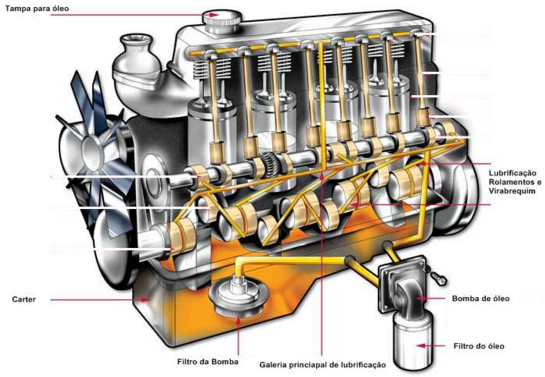
\includegraphics[keepaspectratio=true,scale= 0.7]{figuras/oleomotor.png}
	\caption{Funcionamento e Distribuição do Óleo pelo Motor.}
	\label{fig:oleomotor}
\end{figure}

\subsection{Sistema de Injeção}

	A injeção eletrônica é um sistema de alimentação de combustível e gerenciamento eletrônico de um motor de um veículo automotor. Sua utilização em larga escala se deve à necessidade das indústrias de automóveis reduzirem o índice de emissão de gases poluentes. Esse sistema permite um controle mais eficaz da mistura admitida pelo motor, mantendo-a mais próxima da mistura estequiométrica, mistura de ar/combustível, isso se traduz em maior economia de combustível já que o motor trabalha sempre com a mistura mais adequada e também melhora o desempenho do motor \cite{bosch2004}.
	
	O sistema faz a leitura de diversos sensores espalhados em pontos estratégicos do motor, examina as informações e com base em outras informações gravadas em sua memória envia comandos para diversos atuadores espalhados em pontos estratégicos do motor. Esse procedimento é efetuado varias vezes por minuto com base nos movimentos da cambota.
	
	A cambota ou veio de manivelas transforma uma força num momento binário de forças ou torque. Recebe a força através das biela que são conectadas aos pistões, e transformando-o em momento, transmitido aos demais componentes acoplados nas extremidades de seu eixo.
	
	O sistema de injeção tem como principal componente a Central ou ECU (Engine Control Unit), onde ficam gravadas as informações do veículo e seus parâmetros de fábrica, ela também realiza os cálculos programados para gerenciar a alimentação e ignição do motor. Este sistema também é composto por sensores e atuadores, um esquemático é mostrado a seguir (Figura \ref{fig:oleomotor}) e abaixo serão listados e apresentados os componentes deste sistema \cite{brunetti2012}.
	
\begin{figure}[h!]
	\centering
	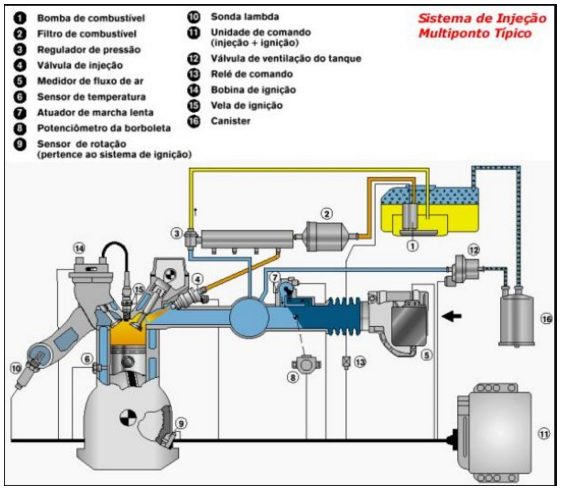
\includegraphics[keepaspectratio=true,scale= 0.7]{figuras/esquematicoinjecao.png}
	\caption{Esquemático do sistema de injeção.}
	\label{fig:oleomotor}
\end{figure}

\begin{itemize}
	\item \textbf{Sensor de Posição da Borboleta de Aceleração}: Este sensor informa à central a posição instantânea da borboleta. Ele é montado junto ao eixo da mesma, e permite à central identificar a potência que o condutor está requerendo do motor, entre outras estratégias de funcionamento.
	\item \textbf{Sensor Temperatura Líquido de Arrefecimento}: Informa à central a temperatura do líquido de arrefecimento, o que é muito importante, pois identifica a temperatura do motor. Enviando um sinal a unidade de comando, que por sua vez altera o tempo de injeção, avanço de ignição, entrada de ar no coletor e até uma dose extra de combustível pelo injetor de partida à frio.
	\item \textbf{Sensor Temperatura Ar}: Este informa à central a temperatura do ar que entra no motor. Junto com o sensor de pressão, a central consegue calcular a massa de ar admitida pelo motor e assim determinar a quantidade de combustível adequada para uma combustão completa.
	\item \textbf{Sensor Pressão do Coletor}: Responsável por informar a diferença de pressão do ar dentro do coletor de admissão, entre a borboleta e o motor, e o ar atmosférico.
Sensor rotação - Informa a central a rotação do motor e na maioria dos sistemas a posição dos êmbolos, para a central realizar o sincronismo da injeção e ignição. Na maioria dos projetos ele é montado acima de uma roda magnética dentada fixada no virabrequim, mas pode ser encontrado em outros eixos também.
	\item \textbf{Sensor Detonação}: Permite a central detectar batidas de pino no interior do motor. Este sensor é fundamental para a vida do motor, já que os motores modernos trabalham em condições críticas, a central diminui o ângulo de avanço de ignição a fim de eliminar o evento denominado como "pré-detonação", tornando a avançá-lo posteriormente, atuando como um corta potência e prevenir uma quebra.
	\item \textbf{Sonda lambda ou Sensor Oxigênio}: Este sensor fica localizado no escapamento do automóvel, ele informa a central a presença de oxigênio nos gases de escape, podendo designar-se por sensor O2 é responsável pelo equilíbrio da injeção, pois ele tem a função de enviar a informação de qual é o estado dos gases da saída do motor e é em função desta informação que a unidade do motor controla o pulso da injeção. Nos automóveis que podem rodar com mais de um combustível ou com uma mistura entre eles, denominados flexfuel, a central consegue identificar o combustível utilizado, ou a mistura entre eles, através do sinal deste sensor.
	\item \textbf{Sensor Velocidade}: Informa a velocidade do automóvel, essencial para várias estratégias da central.
\end{itemize}
	
Os atuadores presentes no sistema de injeção segundo \citeauthor{bosch2004} (\citeyear{bosch2004}) são:

\begin{itemize}
	\item \textbf{Injetores}: Responsáveis pela injeção de combustível no motor, a central controla a quantidade de combustível através do tempo que mantêm o injetor aberto, tempo de injeção. Esses podem ser classificados por seu sistema de funcionamento: monoponto, com apenas um injetor para todos os cilindros ou multiponto, com um injetor por cilindro. Sendo que esses injetam combustível de forma indireta, antes das válvulas de admissão, existe também a injeção direta, que os injetores de combustível injetam dentro da câmara de combustão.
	\item \textbf{Bobinas}: Componente que fornece a faísca para o motor. Os sistemas modernos as ignições estáticas utilizam uma bobina ligada diretamente a dois cilindros ou até uma bobina por cilindro. A central é responsável pelo avanço e sincronismo das faíscas.
	\item \textbf{Motor Corretor Marcha Lenta ou Motor de Passo}: Utilizado para permitir uma entrada de ar suficiente para que o motor mantenha a marcha lenta, indiferente às exigências do ar-condicionado, alternador e outros que possam afetar sua estabilidade. Normalmente o atuador é instalado em um desvio \textit{by pass} da borboleta, podendo controlar o fluxo de ar enquanto ela se encontra em repouso.
	\item \textbf{Bomba de Combustível}: Responsável por fornecer o combustível sob pressão aos injetores. Na maioria dos sistemas é instalada dentro do tanque de combustível do automóvel, ela bombeia o combustível de forma constante e pressurizada, passando pelo filtro de combustível até chegar aos injetores.
	\item \textbf{Válvula Purga Canister}: Permite a circulação dos gases gerados no reservatório de combustível para o motor. Normalmente é acionada com motor em alta exigência.
	\item \textbf{Eletroventilador de Arrefecimento}: Posicionado atrás do radiador, ele é acionado quando o motor se encontra em uma temperatura alta, gerando passagem de ar pelo radiador mesmo quando o automóvel estiver parado.
	\item \textbf{Luz de Avaria do Sistema}: Permite a central avisar ao condutor do automóvel que existe uma avaria no sistema da injeção eletrônica, ela armazena um código de falha referente ao componente e aciona a estratégia de funcionamento para o respectivo componente permitindo que o veículo seja conduzido até um local seguro ou uma oficina. 
\end{itemize}

\section{Caracterização do Motor}

	Para desenvolvimento do projeto foi escolhido o motor Fiat Fiasa para a realização dos testes. É um motor 1.0 MPI geralmente utilizado nos veículos Palio, da montadora Fiat. Os motivos para escolha deste foram principalmente o baixo custo, já que foi fornecido pela universidade, e a melhor adaptação para o tipo de sensoriamento que será realizado.
	
	O nome Fiasa é utilizado para designar uma família de motores Fiat, fabricados no Brasil entre os anos de 1976 e 2001. Inicialmente projetado para o veículo Fiat 147, o motor foi sendo adaptado e otimizado ao longo do tempo a fim de atender à todas exigências do mercado automobilístico. O motor lançado em 1976 era um 4 cilindros de 1049 $cm^3$, tinha 76 mm de diâmetro e 57,8 mm de curso. À época de seu lançamento o motor foi caracterizado como moderno \cite{dantas2012}.
	
\begin{figure}[h!]
	\centering
	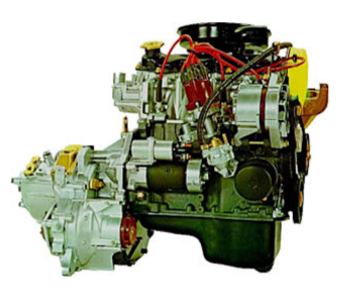
\includegraphics[keepaspectratio=true,scale= 0.7]{figuras/motorfiat.png}
	\caption{Motor Fiat Fiasa.}
	\label{fig:motorfiat}
\end{figure}

	Ainda sobre o primeiro modelo do Fiasa, este era alimentado por um carburador de corpo simples, o que dava uma potência de 51 cv a 6000 rpm e 7,3 m.kgf a 3000 rpm. Nos modelos seguintes o carburador foi substituído por um de corpo duplo, conferindo uma maior potência ao motor.
	
	O motor fabricado no Brasil, ao longo do tempo, passou a ser exportado para equipar carros da Itália, terra natal da montadora Fiat. Isso comprovou a boa qualidade do motor do brasileiro 147.
	
	Com o passar do tempo, o motor Fiasa foi se adaptando, mas não sofreu grandes mudanças. O diâmetro de 76 mm se manteve em todas as versões, e a potência sofreu uma alteração de 26\% de aumento, comparando a primeira versão e a versão final de 2001. O motor inicialmente projetado para o 147, iria equipar no futuro outros modelos da mesma montadora, como o Uno, a Fiorino e o Palio. A partir de 2001, o motor Fiasa de lugar à família de motores Fire, um modelo mais moderno e melhorado, que equipa vários carros da montadora Fiat até o presente momento.
	
	O motor utilizado no projeto em questão é um Fiasa mpi 1.0 que equipava um fiat palio. Este motor possui injeção eletrônica multiponto, potência de 61 cv a 6000 rpm e um torque de 8,1 m.kgf a 3000 rpm. Com a adoção da injeção eletrônica multiponto o motor promoveu uma boa melhora no desempenho do motor. O motor possui todos os seus componentes e está em bom estado, possibilitando a realização dos testes requeridos.
	
\section{Layout do Laboratório}

	As Figuras \ref{fig:sistemaslaboratorio}, \ref{fig:isometricalaboratorio} e \ref{fig:isometricainterna} a seguir ilustram o \textit{layout} do laboratório e todos seus componentes, como também a disposição dos mesmos. A modelagem foi toda realizada no software SolidWorks 3D.
	
\begin{figure}[h!]
	\centering
	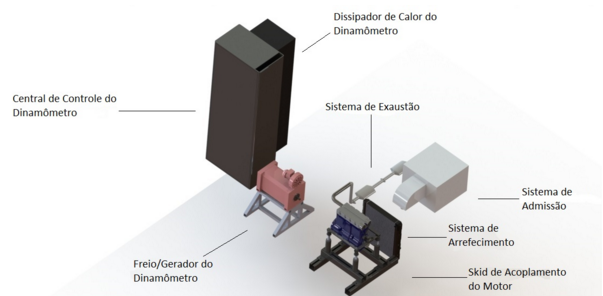
\includegraphics[keepaspectratio=true,scale= 0.4]{figuras/sistemaslaboratorio.png}
	\caption{Disposição dos sistemas do Laboratório.}
	\label{fig:sistemaslaboratorio}
\end{figure}
	
\begin{figure}[h!]
	\centering
	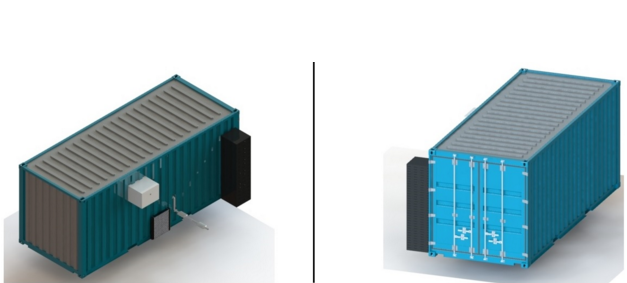
\includegraphics[keepaspectratio=true,scale= 0.35]{figuras/vistaisometricalaboratorio.png}
	\caption{Vista Isométrica da Parte Externa do Laboratório.}
	\label{fig:isometricalaboratorio}
\end{figure}
	
\begin{figure}[h!]
	\centering
	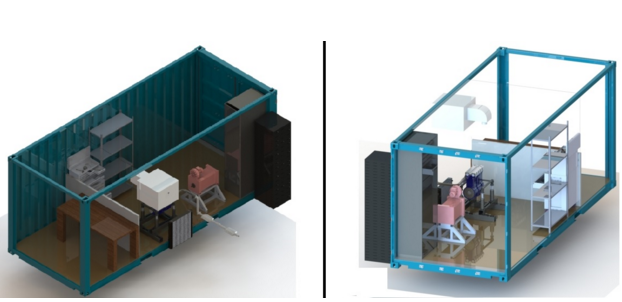
\includegraphics[keepaspectratio=true,scale= 0.4]{figuras/isometricainterna.png}
	\caption{Vista isométrica da parte interna do laboratório.}
	\label{fig:isometricainterna}
\end{figure}

\section{Estrutura de Acoplamento do Motor}

	Para desenvolvimento do nosso projeto será construída uma estrutura para acoplamento do motor, que deve ser capaz de suportar o peso e se adaptar à geometria do mesmo. Serão realizadas simulações numéricas para validação da estrutura, seguido pela sua construção.
	
\begin{figure}[h!]
	\centering
	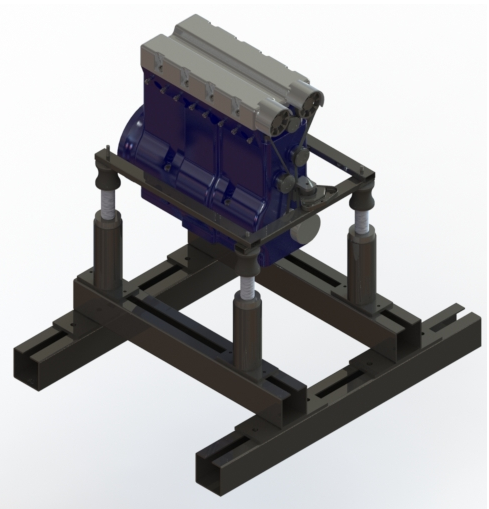
\includegraphics[keepaspectratio=true,scale= 0.4]{figuras/estruturamotor.png}
	\caption{Estrutura de Acoplamento do Motor.}
	\label{fig:estruturamotor}
\end{figure}
